\documentclass[aspectratio=169,10pt]{beamer}
\usepackage{hw1_hud_theme}

\hypersetup{
  pdftitle={PathFinding HCMC — Traffic-Aware A* & ALT Routing | HW1},
  pdfauthor={Group 7 · CC01 · HCMUT},
  pdfsubject={Introduction to Artificial Intelligence (CO3061)},
  colorlinks=true,
  linkcolor=NavCyan,
  urlcolor=NavTeal
}

\begin{document}

% ======================================================================
% SLIDE 01 — COVER
% ======================================================================
\begingroup
\setbeamertemplate{background canvas}{%
  \begin{tikzpicture}[x=1cm,y=1cm]
    \useasboundingbox (0,0) rectangle (16,9);
    \fill[NavBg] (0,0) rectangle (16,9);

    % Right 55% Panel: Crisp Framed Dark HCMC Road Map Showcase
    \fill[NavBorder!15, rounded corners=8pt] (7.38,1.02) rectangle (15.42,7.88);
    \begin{scope}
      \clip[rounded corners=7pt] (7.30,1.10) rectangle (15.34,7.96);
      \fill[black!92] (7.30,1.10) rectangle (15.34,7.96);
      \node[anchor=center, inner sep=0pt] at (11.32,4.53)
        {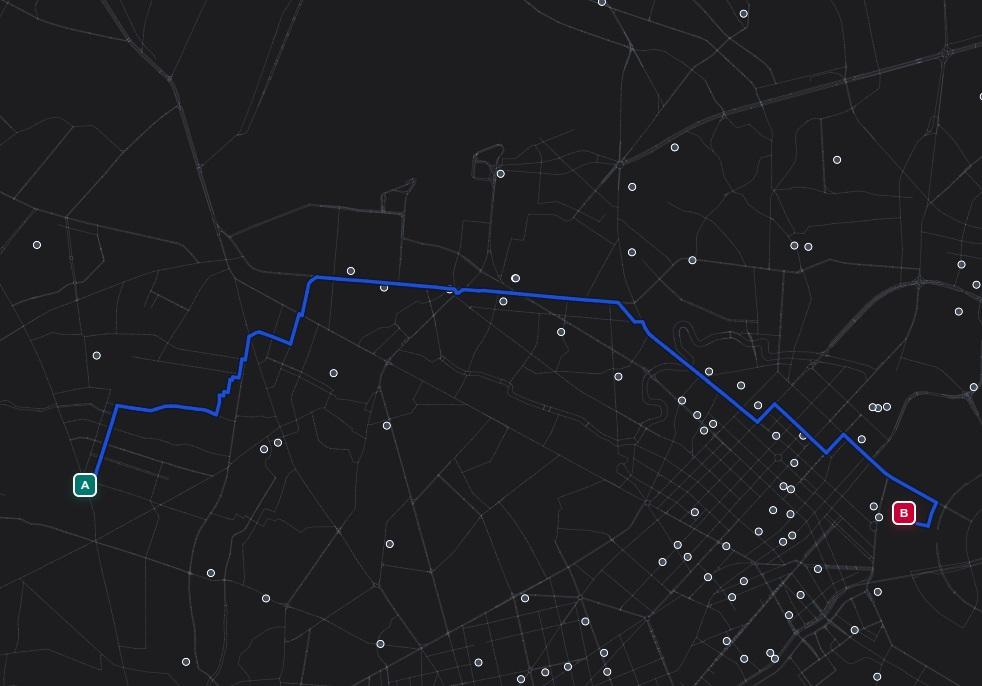
\includegraphics[width=8.60cm]{images/hcmc_cover_map.jpg}};
    \end{scope}
    \draw[NavBorder!55, line width=0.9pt, rounded corners=7pt] (7.30,1.10) rectangle (15.34,7.96);
    \node[anchor=south west, fill=black!78, draw=NavBorder!45, line width=0.5pt,
          rounded corners=3pt, inner xsep=6pt, inner ysep=2.5pt,
          font=\ttfamily\fontsize{6.0}{7.0}\selectfont\bfseries, text=white]
      at (7.52,1.32) {HCMC ROAD GRAPH $\cdot$ 44,178 NODES $\cdot$ 5 VERIFIED HEURISTICS};

    % Cover HUD Corner Brackets
    \draw[NavBorder!70, line width=0.95pt] (0.28,8.28) -- (0.28,8.72) -- (0.72,8.72);
    \draw[NavBorder!70, line width=0.95pt] (15.28,8.72) -- (15.72,8.72) -- (15.72,8.28);
    \draw[NavBorder!70, line width=0.95pt] (0.28,0.72) -- (0.28,0.28) -- (0.72,0.28);
    \draw[NavBorder!70, line width=0.95pt] (15.28,0.28) -- (15.72,0.28) -- (15.72,0.72);
    \fill[NavCyan] (0.28,8.72) circle (0.04) (15.72,8.72) circle (0.04)
                   (0.28,0.28) circle (0.04) (15.72,0.28) circle (0.04);

    % Top-right 4-chip indicator (chip 1 active)
    \node[anchor=east, fill=NavPanel, opacity=0.90, draw=NavBorder!45,
          rounded corners=3pt, inner xsep=6pt, inner ysep=3pt] at (15.15,8.44) {%
      \tikz[x=1cm,y=1cm]{
        \fill[NavCyan, rounded corners=1.2pt] (0,0) rectangle (0.20,0.20);
        \fill[NavTrack, rounded corners=1.2pt] (0.30,0) rectangle (0.50,0.20);
        \fill[NavTrack, rounded corners=1.2pt] (0.60,0) rectangle (0.80,0.20);
        \fill[NavTrack, rounded corners=1.2pt] (0.90,0) rectangle (1.10,0.20);
      }%
    };

    % Top-left HCMUT lockup
    \node[anchor=west, inner sep=0pt] (bk) at (0.85,8.05) {
\includegraphics[height=0.68cm]{images/BK.png}};
    \node[anchor=west, inner sep=0pt, align=left] at (1.72,8.05) {%
      {\fontsize{7.5}{9}\selectfont\bfseries\color{NavIvory}HCMUT $\cdot$ VNU-HCM}\\[2pt]
      {\fontsize{6.8}{8.5}\selectfont\color{NavMuted}Faculty of Computer Science \& Engineering}%
    };

    % Eyebrow pill
    \node[anchor=west, inner sep=0pt] at (0.85,6.88) {\navtag[NavCyan]{GROUP 7 $\cdot$ CC01 $\cdot$ CO3061 $\cdot$ HW1}};

    % Main Cyan/Amber Cinzel Title + Subtitle
    \node[anchor=west, inner sep=0pt, align=left] at (0.82,5.42) {%
      {\navdisplay\fontsize{24}{28}\selectfont\color{NavIvory}PATHFINDING}\\
      {\navdisplay\fontsize{28}{31}\selectfont\color{NavCyan}HCMC}\\[4pt]
      {\navdisplay\fontsize{10.5}{13}\selectfont\color{NavAmber}TRAFFIC-AWARE A* ROUTING}%
    };

    % Diamond divider
    \node[anchor=west, inner sep=0pt] at (0.85,3.82) {\navdivider{4.8}};

    % Cyan tagline
    \node[anchor=west, inner sep=0pt, align=left] at (0.85,3.12) {%
      {\fontsize{11.5}{15}\selectfont\color{NavCyan}Fastest paths.}\\
      {\fontsize{11.5}{15}\selectfont\color{NavCyan}Verified bounds.}%
    };

    % Metadata block (Inter for clean Vietnamese rendering)
    \node[anchor=west, inner sep=0pt, align=left] at (0.85,1.62) {%
      {\fontsize{8.2}{11.5}\selectfont\color{NavMuted}Course: \color{NavIvory}Introduction to Artificial Intelligence (CO3061)}\\
      {\fontsize{8.2}{11.5}\selectfont\color{NavMuted}Advisor: \color{NavIvory}Dr. Nguyễn Quốc Minh}%
    };

    % Cover bottom footer
    \draw[NavBorder!45, line width=0.5pt] (0.85,0.68) -- (6.80,0.68);
    \node[anchor=west, inner sep=0pt, font=\ttfamily\fontsize{6.5}{7.5}\selectfont, text=NavMuted]
      at (0.85,0.42) {PATHFINDING HCMC \ / \ INTRO AI \ $\cdot$ \ HCMUT};
    \node[anchor=east, inner sep=0pt, font=\ttfamily\bfseries\fontsize{8}{9}\selectfont, text=NavCyan]
      at (15.15,0.42) {01};
  \end{tikzpicture}%
}
\begin{frame}[plain]
\mbox{}
\end{frame}
\endgroup

% ======================================================================
% SECTION 01 — PROBLEM & DESIGN (Slides 02–03)
% ======================================================================
\navsetsection{1}{01 / PROBLEM \& DESIGN}
\navgridon

% SLIDE 02 — URBAN ROUTING AS GRAPH SEARCH
\begin{frame}{URBAN ROUTING AS GRAPH SEARCH}
\framesubtitle{Minimum travel time on Ho Chi Minh City's directed road network (shortest distance $\neq$ fastest path)}
\vspace{0.06cm}
\begin{columns}[T,onlytextwidth]
  \begin{column}{5.3cm}
    \navhero[NavCyan]{36}{44,178}\par
    \vspace{2pt}
    {\fontsize{10}{12}\selectfont\bfseries\color{NavAmber}ROAD GRAPH NODES}\par
    \vspace{4pt}
    {\fontsize{8.8}{11.8}\selectfont\color{NavIvory}Travel speed varies across streets and time of day.}\par
    \vspace{5pt}
    \navtag[NavTeal]{103,810 DIRECTED EDGES}\par
    \vspace{6pt}
    \navcardaccent[5.5pt]{NavBorder}{4.7cm}{%
      {\fontsize{7.7}{10.5}\selectfont\color{NavMuted}%
        $\bullet$ \textbf{\color{NavIvory}150 POIs}, \textbf{\color{NavCyan}15 categories} (147 snapped nodes)\\
        $\bullet$ Study box: $\pm 10\text{ km}$ around $(10.7769, 106.7009)$\\
        $\bullet$ One-way streets + parallel edges (\texttt{MultiDiGraph})
      }%
    }
  \end{column}
  \begin{column}{8.6cm}
    \navcard{7.85cm}{%
      \centering
      \begin{tikzpicture}[x=1cm,y=1cm]
        \tikzstyle{gnode}=[fill=NavPanelAlt, draw=NavCyan!80, line width=0.8pt,
                           circle, minimum size=0.60cm,
                           font=\fontsize{8}{9}\selectfont\bfseries, text=NavIvory]
        \node[gnode, draw=NavTeal, fill=NavTeal!14!white, text=NavTeal] (A) at (0.7, 1.85) {A};
        \node[gnode] (u) at (2.8, 2.55) {$u$};
        \node[gnode] (w) at (2.8, 0.95) {$w$};
        \node[gnode] (v) at (5.3, 2.15) {$v$};
        \node[gnode, draw=NavCrimson, fill=NavCrimson!14!white, text=NavCrimson] (B) at (7.1, 1.45) {B};

        \draw[NavCyan, line width=1.1pt, -{Stealth[length=2mm]}] (A) -- node[above left, font=\ttfamily\fontsize{6.8}{8}\selectfont, text=NavMuted] {14s} (u);
        \draw[NavBorder!80, line width=0.85pt, -{Stealth[length=2mm]}] (A) -- node[below left, font=\ttfamily\fontsize{6.8}{8}\selectfont, text=NavMuted] {22s} (w);

        % Parallel edges u -> v
        \draw[NavAmber, line width=0.95pt, bend left=26, -{Stealth[length=2mm]}]
          (u) to node[above, font=\ttfamily\fontsize{6.6}{8}\selectfont, text=NavAmber] {k=0: 42s (slow)} (v);
        \draw[NavCyan, line width=1.25pt, bend right=18, -{Stealth[length=2mm]}]
          (u) to node[below, yshift=-1pt, font=\ttfamily\fontsize{6.6}{8}\selectfont\bfseries, text=NavCyan] {k=1: 19s (fast)} (v);

        \draw[NavBorder!80, line width=0.85pt, -{Stealth[length=2mm]}] (w) -- node[below right, font=\ttfamily\fontsize{6.8}{8}\selectfont, text=NavMuted] {28s} (v);
        \draw[NavCyan, line width=1.1pt, -{Stealth[length=2mm]}] (v) -- node[above right, font=\ttfamily\fontsize{6.8}{8}\selectfont, text=NavMuted] {12s} (B);

        % Formula strip
        \node[fill=NavPanelAlt, draw=NavBorder!45, rounded corners=3pt, inner xsep=8pt, inner ysep=3.5pt,
              font=\ttfamily\fontsize{7.5}{9}\selectfont, text=NavAmber]
          at (3.9, 0.15) {c(e) = 3.6 * L\_e / v\_e \ (seconds), \ \ v\_e > 0};
      \end{tikzpicture}
    }
  \end{column}
\end{columns}
\end{frame}

% SLIDE 03 — SYSTEM ARCHITECTURE & TRAFFIC PIPELINE
\navgridoff
\begin{frame}{SYSTEM ARCHITECTURE \& TRAFFIC PIPELINE}
\navslidetag[NavCyan]{DESIGN $\cdot$ UNIFIED ENGINE}
\framesubtitle{Three-stage pipeline from OSMnx + Kaggle speeds to verified 5-heuristic A* and FIFO time-dependent routing}
\vspace{0.08cm}

\noindent\begin{tikzpicture}[x=1cm,y=1cm]
  \useasboundingbox (0,0) rectangle (14.3,1.95);
  \node[fill=NavPanel, draw=NavBorder!45, rounded corners=5pt, inner sep=7pt,
        text width=3.65cm, minimum height=1.68cm, anchor=west, text=NavIvory] (c1) at (0,0.98) {%
    {\ttfamily\fontsize{6.8}{8}\selectfont\bfseries\color{NavAmber}01 $\cdot$ DATA \& TRAFFIC}\\[3pt]
    {\fontsize{10.2}{12.5}\selectfont\bfseries\color{NavIvory}OSMnx +}\\
    {\fontsize{10.2}{12.5}\selectfont\bfseries\color{NavIvory}Kaggle HCMC}\\[2pt]
    {\fontsize{7.3}{9.2}\selectfont\color{NavMuted}Median speed (5--100\,km/h) + 5-tier fallback}%
  };
  \draw[NavCyan, line width=1.1pt, -{Stealth[length=2.2mm]}] (4.18,0.98) -- (4.88,0.98);

  \node[fill=NavPanelAlt, draw=NavCyan!65, line width=0.9pt, rounded corners=5pt, inner sep=7pt,
        text width=3.95cm, minimum height=1.68cm, anchor=west, text=NavIvory] (c2) at (4.94,0.98) {%
    {\ttfamily\fontsize{6.8}{8}\selectfont\bfseries\color{NavCyan}02 $\cdot$ UNIFIED A* ENGINE}\\[3pt]
    {\fontsize{10.2}{12.5}\selectfont\bfseries\color{NavIvory}5 Verified Heuristics}\\
    {\fontsize{10.2}{12.5}\selectfont\bfseries\color{NavIvory}+ FIFO Time Routing}\\[2pt]
    {\fontsize{7.3}{9.2}\selectfont\color{NavMuted}Zero, Safe, Edge-Local, Sep/Joint ALT}%
  };
  \draw[NavCyan, line width=1.1pt, -{Stealth[length=2.2mm]}] (9.42,0.98) -- (10.10,0.98);

  \node[fill=NavPanel, draw=NavBorder!45, rounded corners=5pt, inner sep=7pt,
        text width=3.55cm, minimum height=1.68cm, anchor=west, text=NavIvory] (c3) at (10.14,0.98) {%
    {\ttfamily\fontsize{6.8}{8}\selectfont\bfseries\color{NavTeal}03 $\cdot$ UI \& AUDIT}\\[3pt]
    {\fontsize{10.2}{12.5}\selectfont\bfseries\color{NavIvory}MapLibre/Leaflet}\\
    {\fontsize{10.2}{12.5}\selectfont\bfseries\color{NavIvory}+ NetworkX Audit}\\[2pt]
    {\fontsize{7.3}{9.2}\selectfont\color{NavMuted}GeoJSON routes + rev.-Dijkstra check}%
  };
\end{tikzpicture}\par

\vspace{0.08cm}
\noindent\navdivider{14.3}\par
\vspace{0.08cm}

\begin{columns}[T,onlytextwidth]
  \begin{column}{6.95cm}
    \navcardaccent[7pt]{NavAmber}{6.22cm}{%
      {\ttfamily\fontsize{7.0}{8.2}\selectfont\bfseries\color{NavAmber}FROZEN SNAPSHOT + FIFO TIME SUPPORT}\\[3pt]
      {\fontsize{8.0}{10.8}\selectfont\color{NavIvory}Static benchmarks use frozen \texttt{weekday 08:00--08:29}. Time-dependent FIFO routing (\texttt{src/time\_routing.py}) supports \textbf{Safe} \& \textbf{Zero} across periods with snapshot guards.}%
    }
  \end{column}
  \begin{column}{6.95cm}
    \navcardaccent[7pt]{NavCyan}{6.22cm}{%
      {\ttfamily\fontsize{7.0}{8.2}\selectfont\bfseries\color{NavCyan}KEYED MULTIGRAPH, ACCESS \& 44 TESTS}\\[3pt]
      {\fontsize{8.0}{10.8}\selectfont\color{NavIvory}Parent pointers store \texttt{(u, key)} for parallel edges. POI-to-road access legs are separated from driving cost. Verified by \textbf{44 unit tests} across \textbf{9 test modules}.}%
    }
  \end{column}
\end{columns}
\end{frame}

% ======================================================================
% SECTION 02 — ALGORITHMS & PROOFS (Slides 04–06)
% ======================================================================
\navsetsection{2}{02 / ALGORITHMS \& PROOFS}
\navgridon

% SLIDE 04 — CUSTOM A* & SAFE HEURISTIC PROOF
\begin{frame}{CUSTOM A* \& SAFE HEURISTIC PROOF}
\navslidetag[NavTeal]{ADMISSIBLE \& CONSISTENT}
\framesubtitle{Keyed $f(n)=g(n)+h(n)$ search with global speed bound $V_{\mathrm{upper}}$ and exhaustive edge-bound verification}
\vspace{0.06cm}
\begin{columns}[T,onlytextwidth]
  \begin{column}{7.85cm}
    \navcard[inner sep=7.5pt]{7.15cm}{%
      {\ttfamily\fontsize{7.0}{8.2}\selectfont\bfseries\color{NavCyan}SAFE HEURISTIC BOUND \& CONSISTENCY PROOF}\\[3pt]
      {\fontsize{8.1}{10.8}\selectfont\color{NavIvory}%
        \[
          V_{\mathrm{upper}}(S) = 1.001 \max_{e \in E} v_e(S) = \mathbf{74.074\;\mathrm{km/h}}, \quad
          h_{\mathrm{safe}}(n,t;S) = \frac{3.6\,d_{\mathrm{hav}}(n,t)}{V_{\mathrm{upper}}(S)}
        \]
        \textbf{Load-time edge check} ($\forall$ traversable $(u,v)$):
        \[
          c(u,v) \ge \frac{3.6\,d_{\mathrm{hav}}(u,v)}{V_{\mathrm{upper}}(S)}
        \]
        By great-circle triangle inequality:
        \[
          h_{\mathrm{safe}}(u,t) \le \frac{3.6\,d_{\mathrm{hav}}(u,v)}{V_{\mathrm{upper}}(S)} + h_{\mathrm{safe}}(v,t) \le c(u,v) + h_{\mathrm{safe}}(v,t)
        \]
        \centering\textbf{\color{NavTeal}Consistent $\Longrightarrow$ Admissible $\Longrightarrow$ Optimal A*}%
      }%
    }
  \end{column}
  \begin{column}{5.95cm}
    \navcardaccent[6.5pt]{NavTeal}{5.25cm}{%
      \navhero[NavTeal]{21}{0 / 103,810}\par
      \vspace{1pt}
      {\ttfamily\fontsize{7.0}{8.2}\selectfont\bfseries\color{NavTeal}EDGE-BOUND VIOLATIONS}\\[3pt]
      {\fontsize{7.9}{10.6}\selectfont\color{NavIvory}%
        $\bullet$ Min margin: \textbf{\color{NavTeal}0.064892\,s} (strict check)\\
        $\bullet$ Graph stays frozen after validation%
      }%
    }\par
    \vspace{0.12cm}
    \navcardaccent[6.5pt]{NavCyan}{5.25cm}{%
      {\ttfamily\fontsize{7.0}{8.2}\selectfont\bfseries\color{NavCyan}CUSTOM A* IMPLEMENTATION}\\[3pt]
      {\fontsize{7.9}{10.8}\selectfont\color{NavIvory}%
        \navcheck\ \ Min-heap $f(n)=g(n)+h(n)$\\
        \navcheck\ \ Keyed \texttt{(parent, key)} for parallel edges\\
        \navcheck\ \ Node reopening on cheaper $g(n)$\\
        \navcheck\ \ Explicit \texttt{no-route} if disconnected%
      }%
    }
  \end{column}
\end{columns}
\end{frame}

% SLIDE 05 — FIXING LOCAL TRAFFIC: EDGE-BASED LOOKAHEAD
\begin{frame}{FIXING LOCAL TRAFFIC: EDGE-BASED LOOKAHEAD}
\navslidetag[NavTeal]{BEFORE VS AFTER}
\framesubtitle{Replacing broken congestion scaling ($\beta=0.25$) with Bellman-consistent one-step edge lookahead}
\vspace{0.06cm}
\begin{columns}[T,onlytextwidth]
  \begin{column}{6.85cm}
    \navcardaccent[6.5pt]{NavCrimson}{6.15cm}{%
      {\ttfamily\fontsize{7.0}{8.2}\selectfont\bfseries\color{NavCrimson}BEFORE $\cdot$ LEGACY MEAN-TRAFFIC ($\beta=0.25$)}\\[3pt]
      {\fontsize{7.8}{10.5}\selectfont\color{NavIvory}%
        $h_{\mathrm{traffic}}(n,t) = h_{\mathrm{safe}}(n,t)\,[1 + 0.25\,q_S(n)]$
      }\\[4pt]
      \centering
      \begin{tikzpicture}[x=1cm,y=1cm]
        \node[circle, draw=NavCrimson, fill=NavPanelAlt, minimum size=0.52cm, font=\fontsize{8}{9}\selectfont\bfseries] (u) at (0.6,0.9) {$u$};
        \node[circle, draw=NavTeal, fill=NavPanelAlt, minimum size=0.52cm, font=\fontsize{8}{9}\selectfont\bfseries] (t) at (4.4,0.9) {$t$};
        \draw[NavCyan, line width=1pt, -{Stealth[length=1.8mm]}] (u) -- node[above, font=\ttfamily\fontsize{7}{8}\selectfont\bfseries] {c(u,t)=10.00\,s} (t);
        \node[fill=NavPanelAlt, draw=NavCrimson!45, rounded corners=3pt, inner sep=3pt, align=left,
              font=\ttfamily\fontsize{6.6}{8.4}\selectfont, text=NavIvory] at (2.5,0.12) {%
          h\_safe=9.99\,s, q\_S=0.50 $\Rightarrow$ \color{NavCrimson}\bfseries 11.24\,s > 10.00\,s \navcross%
        };
      \end{tikzpicture}\\[3pt]
      \raggedright{\fontsize{7.8}{10.5}\selectfont\color{NavIvory}%
        $\bullet$ \textbf{\color{NavCrimson}115,612} consistency violations (12 goals)\\
        $\bullet$ Max excess \textbf{158.72\,s} (POI 29); breaks optimality%
      }%
    }
  \end{column}
  \begin{column}{6.85cm}
    \navcardaccent[6.5pt]{NavTeal}{6.15cm}{%
      {\ttfamily\fontsize{7.0}{8.2}\selectfont\bfseries\color{NavTeal}AFTER $\cdot$ EDGE-BASED LOOKAHEAD ($h_{\mathrm{edge}}$)}\\[3pt]
      {\fontsize{7.8}{10.5}\selectfont\color{NavIvory}%
        \[
          h_{\mathrm{edge}}(n,t) = \begin{cases}
            0, & n = t \\
            h_{\mathrm{safe}}(n,t), & \text{dead end} \\
            \min_{e=(n,v)} \bigl[c_S(e) + h_{\mathrm{safe}}(v,t)\bigr], & \text{otherwise}
          \end{cases}
        \]
        \textbf{Bellman + Safe consistency proof:}\\
        $h_{\mathrm{edge}}(u,t) \le c_S(u,v) + h_{\mathrm{safe}}(v,t) \le c_S(u,v) + h_{\mathrm{edge}}(v,t)$\\[2pt]
        \navcheck\ \ $h_{\mathrm{safe}} \le h_{\mathrm{edge}} \le h^*$ \textbf{(0 adm / 0 cons violations)}%
      }%
    }
  \end{column}
\end{columns}\par
\vspace{0.10cm}
\navcardaccent[5.5pt]{NavCyan}{13.55cm}{%
  {\fontsize{8.0}{10.5}\selectfont\color{NavIvory}%
    \textbf{\color{NavCyan}Key insight:} Taking $\min$ over actual outgoing edge costs $c_S(e)$ estimates remaining travel time without double-counting congestion.%
  }%
}
\end{frame}

% SLIDE 06 — LANDMARK ACCELERATION: JOINT & SEPARATE ALT
\begin{frame}{LANDMARK ACCELERATION: JOINT \& SEPARATE ALT}
\navslidetag[NavViolet]{ALT $\cdot$ TRIANGLE INEQUALITY}
\framesubtitle{Directed landmark lower bounds tighten $h$ from $0.533$ to $0.957$ while preserving exact optimality}
\vspace{0.04cm}

\navcardaccent[5pt]{NavBorder}{13.55cm}{%
  {\fontsize{7.8}{10}\selectfont\color{NavIvory}%
    \textbf{\color{NavCyan}Edge-Cost Decomposition:} \ $c_S(e) = c_{\mathrm{free}}(e) + c_{\mathrm{delay}}(e)$, \ where \ $c_{\mathrm{free}}(e) = \min\!\left(c_S(e),\;\frac{3.6\,L_e}{v_{\mathrm{free}}(e)}\right)$ \ and \ $c_{\mathrm{delay}}(e) = c_S(e) - c_{\mathrm{free}}(e) \ge 0$.%
  }%
}\par
\vspace{0.10cm}

\begin{columns}[T,onlytextwidth]
  \begin{column}{6.85cm}
    \navcardaccent[6.5pt]{NavViolet}{6.15cm}{%
      {\ttfamily\fontsize{7.0}{8.2}\selectfont\bfseries\color{NavViolet}JOINT ALT (DIRECT $c_S$ BOUND)}\\[2pt]
      {\fontsize{7.8}{10.4}\selectfont\color{NavIvory}%
        \[
          h_{\mathrm{joint}}(n,t) = \max_{\ell \in L}\max\bigl(d_S(\ell,t)-d_S(\ell,n),\; d_S(n,\ell)-d_S(t,\ell),\; 0\bigr)
        \]
        $\bullet$ Combined with $h_{\mathrm{safe}}$; single distance table per landmark\\
        $\bullet$ \textbf{\color{NavViolet}Half the cache} (\texttt{26.6\,KB}) \& tighter on 95.0\% of pairs%
      }%
    }
  \end{column}
  \begin{column}{6.85cm}
    \navcardaccent[6.5pt]{NavIndigo}{6.15cm}{%
      {\ttfamily\fontsize{7.0}{8.2}\selectfont\bfseries\color{NavIndigo}SEPARATE DELAY ALT (DECOMPOSED)}\\[2pt]
      {\fontsize{7.8}{10.4}\selectfont\color{NavIvory}%
        \[
          h_{\mathrm{sep}}(n,t) = h_{\mathrm{free}}(n,t) + h_{\mathrm{delay}}(n,t)
        \]
        $\bullet$ Independent ALT bounds on $c_{\mathrm{free}}$ and $c_{\mathrm{delay}}$\\
        $\bullet$ \textbf{\color{NavIndigo}Dual tables} (\texttt{53.0\,KB}); isolates congestion delay bound%
      }%
    }
  \end{column}
\end{columns}\par
\vspace{0.10cm}

\navcardaccent[5.5pt]{NavCyan}{13.55cm}{%
  {\fontsize{7.8}{10.4}\selectfont\color{NavIvory}%
    \textbf{\color{NavCyan}Directed Safety \& Custom Landmarks:} Unreachable distances use finite caps $M_F, M_R$ (no $\infty - \infty$); defaults to Tan Son Nhat Airport or \textbf{1--32 custom} / \textbf{4, 8, 16, 32 auto} landmarks with \textbf{SHA-256 LRU cache}.%
  }%
}
\end{frame}

% ======================================================================
% SECTION 03 — EXPERIMENTAL RESULTS (Slides 07–10)
% ======================================================================
\navsetsection{3}{03 / EXPERIMENTAL RESULTS}
\navgridoff

% SLIDE 07 — FULL HCMC GRAPH: SAFE CUTS EXPANSIONS 46.1%
\begin{frame}{FULL HCMC GRAPH: SAFE CUTS EXPANSIONS 46.1\%}
\navslidetag[NavCyan]{SCOPE A $\cdot$ 44.2K NODES}
\framesubtitle{Archived v0.3.0 evaluation (seed 42, 20 pairs, 12 goals, weekday 08:00--08:29): all 20/20 match Dijkstra}
\vspace{0.06cm}
\begin{columns}[T,onlytextwidth]
  \begin{column}{4.85cm}
    \vspace{0.04cm}
    \navhero[NavCyan]{36}{46.1\%}\par
    \vspace{2pt}
    {\fontsize{9.4}{11.5}\selectfont\bfseries\color{NavAmber}FEWER EXPANDED NODES}\par
    \vspace{2pt}
    {\fontsize{8.3}{10.5}\selectfont\color{NavIvory}Safe A* vs Zero baseline}\par
    \vspace{6pt}
    \navtag[NavTeal]{20/20 DIJKSTRA MATCHES}\par
    \vspace{7pt}
    \navcardaccent[6pt]{NavBorder}{4.3cm}{%
      {\fontsize{7.6}{10.5}\selectfont\color{NavMuted}%
        $\bullet$ \textbf{\color{NavIvory}Audit:} 12 goals $\times$ 44,022 reachable nodes (rev. Dijkstra)\\
        $\bullet$ \textbf{\color{NavIvory}Tolerance:} $10^{-6}\text{ s}$\\
        $\bullet$ \textbf{\color{NavAmber}POI 118$\to$138:} Legacy Traffic took \textbf{+2,345} extra nodes vs Safe (27,114 vs 24,769)%
      }%
    }
  \end{column}
  \begin{column}{8.95cm}
    \navcard[inner sep=7pt]{8.20cm}{%
      \navbar{Zero (Dijkstra)}{2.75}{3.55}{1.000}{192,099}{NavStone}\\[5pt]
      \navbar{Legacy Traffic}{2.75}{3.55}{0.546}{104,846}{NavAmber}\\[5pt]
      \navbar{Safe A*}{2.75}{3.55}{0.539}{103,510}{NavCyan}\\[4pt]
      {\ttfamily\fontsize{6.2}{7.8}\selectfont\color{NavMuted}TOTAL EXPANDED NODES (20 PAIRS) $\cdot$ SAFE SAVES 33.2\%--60.1\% PER PAIR}%
    }\par
    \vspace{0.10cm}
    \navcard[inner sep=5.5pt]{8.20cm}{%
      \setlength{\tabcolsep}{4pt}%
      \renewcommand{\arraystretch}{1.05}%
      \fontsize{7.5}{9.0}\selectfont
      \begin{tabular}{@{}>{\bfseries\color{NavIvory}}p{2.15cm}>{\centering\arraybackslash\color{NavIvory}}p{1.40cm}>{\centering\arraybackslash\color{NavIvory}}p{1.85cm}>{\color{NavMuted}}p{1.55cm}@{}}
        \toprule
        \textbf{\color{NavMuted}Heuristic} & \textbf{\color{NavMuted}Adm. Viol.} & \textbf{\color{NavMuted}Cons. Viol.} & \textbf{\color{NavMuted}Guarantee} \\
        \midrule
        Safe & \color{NavTeal}\textbf{0} & \color{NavTeal}\textbf{0} & \color{NavTeal}Proven \\
        Legacy Traffic & 0* & \color{NavCrimson}\textbf{115,612} & \color{NavAmber}Sampled* \\
        Zero & 0 & 0 & Baseline \\
        \bottomrule
      \end{tabular}%
    }\par
    \vspace{0.06cm}
    {\fontsize{6.8}{8.5}\selectfont\color{NavMuted}*Scope A: Archived v0.3.0 full 44,178-node graph (\texttt{report/evaluation-summary.json}).}%
  \end{column}
\end{columns}
\end{frame}

% SLIDE 08 — 5-METHOD BENCHMARK: EXPANSIONS & TIGHTNESS
\begin{frame}{5-METHOD BENCHMARK: EXPANSIONS \& TIGHTNESS}
\navslidetag[NavViolet]{SCOPE B $\cdot$ 150 HCMC PLACES}
\framesubtitle{Controlled 5-method benchmark (150 nodes, 990 edges, 8 landmarks, seed 42, 20 pairs, 12 goals)}
\vspace{0.05cm}
\begin{columns}[T,onlytextwidth]
  \begin{column}{4.35cm}
    \navhero[NavViolet]{34}{-80.7\%}\par
    \vspace{1pt}
    {\fontsize{9.0}{11}\selectfont\bfseries\color{NavViolet}JOINT ALT EXPANSIONS}\par
    \vspace{2pt}
    {\fontsize{8.0}{10.2}\selectfont\color{NavIvory}14.80 vs 76.75 (Zero baseline)}\par
    \vspace{6pt}
    \navcardaccent[6pt]{NavTeal}{3.80cm}{%
      \navhero[NavTeal]{24}{0.957}\par
      {\ttfamily\fontsize{6.6}{7.8}\selectfont\bfseries\color{NavTeal}MEAN TIGHTNESS ($h/h^*$)}\\[3pt]
      {\fontsize{7.6}{10}\selectfont\color{NavIvory}%
        \navcheck\ \ \textbf{0 / 0} adm. \& cons. violations across all 5 methods\\
        \navcheck\ \ \textbf{20 / 20} exact Dijkstra matches (mean cost \texttt{1054.442\,s})%
      }%
    }
  \end{column}
  \begin{column}{9.45cm}
    \navcard[inner sep=6pt]{8.75cm}{%
      \navbar{Zero (Dijkstra)}{2.45}{4.20}{1.000}{76.75}{NavStone}\\[3.5pt]
      \navbar{Safe A*}{2.45}{4.20}{0.571}{43.85}{NavCyan}\\[3.5pt]
      \navbar{Edge-Local}{2.45}{4.20}{0.534}{40.95}{NavAmber}\\[3.5pt]
      \navbar{Separate ALT}{2.45}{4.20}{0.334}{25.60}{NavIndigo}\\[3.5pt]
      \navbar{Joint ALT}{2.45}{4.20}{0.193}{14.80}{NavViolet}%
    }\par
    \vspace{0.08cm}
    \navcard[inner sep=5pt]{8.75cm}{%
      \setlength{\tabcolsep}{3.5pt}%
      \renewcommand{\arraystretch}{1.04}%
      \fontsize{7.2}{8.6}\selectfont
      \begin{tabular}{@{}>{\bfseries\color{NavIvory}}p{2.15cm}ccccc@{}}
        \toprule
        \textbf{\color{NavMuted}Method} & \textbf{\color{NavMuted}Mean Exp.} & \textbf{\color{NavMuted}vs Zero} & \textbf{\color{NavMuted}Query} & \textbf{\color{NavMuted}Tight.} & \textbf{\color{NavMuted}Viol. / Match} \\
        \midrule
        Zero & 76.75 & -- & 0.728\,ms & 0.0000 & \color{NavTeal}0/0 $\cdot$ 20/20 \\
        Safe & 43.85 & $-$42.9\% & 0.571\,ms & 0.5334 & \color{NavTeal}0/0 $\cdot$ 20/20 \\
        Edge-Local & 40.95 & $-$46.6\% & 1.718\,ms & 0.6056 & \color{NavTeal}0/0 $\cdot$ 20/20 \\
        Separate ALT & 25.60 & $-$66.6\% & 0.601\,ms & 0.8016 & \color{NavTeal}0/0 $\cdot$ 20/20 \\
        Joint ALT & \color{NavViolet}\textbf{14.80} & \color{NavViolet}\textbf{$-$80.7\%} & \color{NavTeal}\textbf{0.285\,ms} & \color{NavViolet}\textbf{0.9565} & \color{NavTeal}0/0 $\cdot$ 20/20 \\
        \bottomrule
      \end{tabular}%
    }
  \end{column}
\end{columns}
\end{frame}

% SLIDE 09 — COMPUTATIONAL TRADE-OFFS: QUERY VS OVERHEAD
\begin{frame}{COMPUTATIONAL TRADE-OFFS: QUERY VS OVERHEAD}
\navslidetag[NavAmber]{PLACES + GRID BENCHMARKS}
\framesubtitle{Tighter bounds do not always mean faster queries: outgoing-edge scans vs precomputed ALT tables}
\vspace{0.06cm}
\begin{columns}[T,onlytextwidth]
  \begin{column}{6.85cm}
    \navcardaccent[6.5pt]{NavAmber}{6.15cm}{%
      {\ttfamily\fontsize{7.0}{8.2}\selectfont\bfseries\color{NavAmber}EDGE-LOCAL VS SAFE A*}\\[4pt]
      {\fontsize{8.0}{11}\selectfont\color{NavIvory}%
        $\bullet$ \textbf{Fewer nodes:} \textbf{$-$6.6\%} on Places (\texttt{40.95} vs \texttt{43.85}) and \textbf{$-$15.3\%} on 144-Grid (\texttt{38.80} vs \texttt{45.80}); \textbf{0} Safe-dominance violations.\\[3pt]
        $\bullet$ \textbf{\color{NavAmber}Slower query:} \texttt{1.718\,ms} vs \texttt{0.571\,ms} (Places) and \texttt{0.894\,ms} vs \texttt{0.424\,ms} (Grid) due to per-expansion outgoing-edge scan (\texttt{1.301\,ms} heur vs \texttt{0.146\,ms}).%
      }%
    }
  \end{column}
  \begin{column}{6.85cm}
    \navcardaccent[6.5pt]{NavViolet}{6.15cm}{%
      {\ttfamily\fontsize{7.0}{8.2}\selectfont\bfseries\color{NavViolet}JOINT ALT VS SEPARATE ALT}\\[4pt]
      {\fontsize{8.0}{11}\selectfont\color{NavIvory}%
        $\bullet$ \textbf{Tightness (Places, 1,788 pairs):} Joint > Sep \textbf{\color{NavViolet}95.0\%} (\texttt{1,699}), Sep > Joint \texttt{2.7\%} (\texttt{49}), Equal \texttt{2.2\%} (\texttt{40}).\\[2pt]
        $\bullet$ \textbf{Tightness (Grid, 1,716 pairs):} Joint > Sep \textbf{\color{NavViolet}63.3\%} (\texttt{1,087}), Sep > Joint \texttt{8.9\%} (\texttt{152}), Equal \texttt{27.8\%} (\texttt{477}).\\[2pt]
        $\bullet$ \textbf{Preprocess \& Cache:} Joint \texttt{17.5\,ms / 26.6\,KB} vs Separate \texttt{27.8\,ms / 53.0\,KB} (Places).%
      }%
    }
  \end{column}
\end{columns}\par
\vspace{0.12cm}
\navcardaccent[6pt]{NavTeal}{13.55cm}{%
  {\fontsize{8.0}{10.8}\selectfont\color{NavIvory}%
    \textbf{\color{NavTeal}Practical Selection:} Use \textbf{Safe A*} for zero preprocessing or FIFO time-routing; \textbf{Joint ALT} for fastest static queries (\texttt{0.285\,ms}) \& smallest cache; \textbf{Separate ALT} to isolate free-flow vs delay bounds.%
  }%
}
\end{frame}

% SLIDE 10 — INTERACTIVE MAP UI & ROUTE CASE STUDY
\begin{frame}{INTERACTIVE MAP UI \& ROUTE CASE STUDY}
\navslidetag[NavCyan]{WEB UI $\cdot$ POI 132 $\to$ 121}
\framesubtitle{Archived full-graph case study (Bách Hóa Xanh $\to$ Bến Thủ Thiêm) + upgraded 5-method MapLibre UI}
\vspace{0.06cm}
\begin{columns}[T,onlytextwidth]
  \begin{column}{8.20cm}
    \begin{tikzpicture}[x=1cm,y=1cm]
      \node[anchor=south west, inner sep=1pt, draw=NavBorder!55, line width=0.8pt,
            fill=NavPanel, rounded corners=4pt] (shot) at (0,0)
        {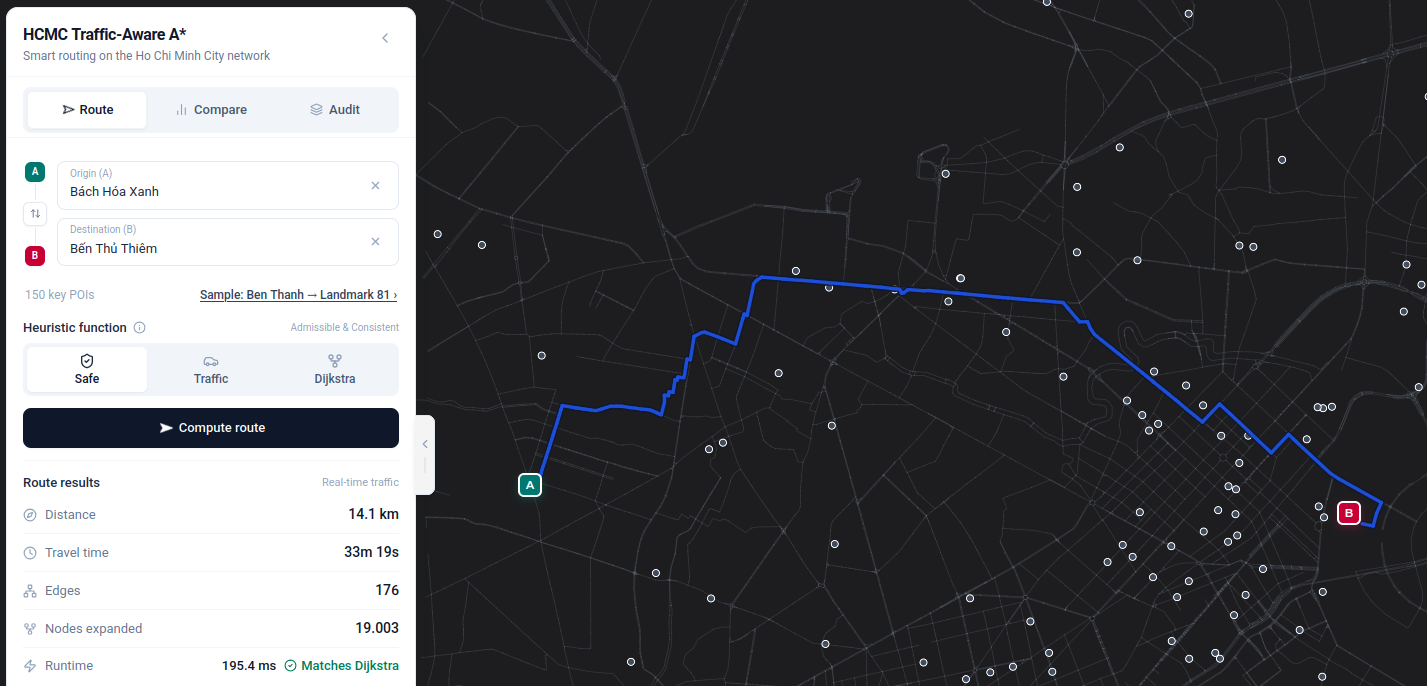
\includegraphics[width=7.90cm]{images/qa_1.png}};
      \node[anchor=south, inner sep=2pt, draw=NavCyan, line width=1.1pt,
            fill=white, rounded corners=4pt] (loupe) at (4.95,0.12)
        {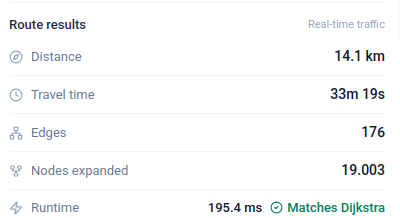
\includegraphics[width=2.65cm]{images/qa_safe_zoom.png}};
      \node[anchor=south east, fill=NavCyan, draw=NavCyan, line width=0.6pt,
            rounded corners=2pt, inner xsep=4pt, inner ysep=1.5pt,
            font=\ttfamily\fontsize{5.5}{6.5}\selectfont\bfseries, text=white]
        at ($(loupe.north east)+(-0.04,-0.02)$) {ZOOM $\cdot$ SAFE METRICS};
      \draw[NavCyan, line width=0.9pt, dashed, -{Stealth[length=1.8mm]}]
        (2.10,0.85) -- (loupe.west);
    \end{tikzpicture}
  \end{column}
  \begin{column}{5.70cm}
    \navcardaccent[5pt]{NavCyan}{5.05cm}{%
      {\ttfamily\fontsize{6.6}{7.8}\selectfont\bfseries\color{NavCyan}ARCHIVED CASE STUDY (SAFE VS LEGACY)}\\[1.5pt]
      {\fontsize{7.8}{10.2}\selectfont\color{NavIvory}%
        \textbf{Safe:} \texttt{19,003} nodes (\texttt{195.4\,ms*}) $\cdot$ \textbf{14.1\,km} (\texttt{14.094\,km}) $\cdot$ \textbf{33m\,19s} (\texttt{1,999.363\,s}) $\cdot$ \texttt{176} edges $\cdot$ Matches Dijkstra\\[2pt]
        \textbf{Legacy Traffic:} \texttt{19,857} nodes (\textbf{+4.49\%}, \texttt{373.4\,ms*})%
      }%
    }\par\vspace{5pt}
    \navcardaccent[5pt]{NavViolet}{5.05cm}{%
      {\ttfamily\fontsize{6.6}{7.8}\selectfont\bfseries\color{NavViolet}UPGRADED REACT + MAPLIBRE UI}\\[1.5pt]
      {\fontsize{7.6}{10.2}\selectfont\color{NavIvory}%
        $\bullet$ Supports all \textbf{5 verified heuristics}\\
        $\bullet$ \textbf{Custom Landmarks} (click map / presets, 1--32)\\
        $\bullet$ \texttt{--demo} mode for interactive benchmark exploration%
      }%
    }\par\vspace{5pt}
    \navcardaccent[5pt]{NavMuted}{5.05cm}{%
      {\ttfamily\fontsize{6.4}{7.4}\selectfont\bfseries\color{NavMuted}TRANSPARENCY NOTE}\\[1.5pt]
      {\fontsize{7.1}{9.3}\selectfont\color{NavMuted}*Screenshot is from archived v0.3.0 full-graph UI (single run). \texttt{--demo} mode uses simulated fixtures, separate from the 44.2k graph.}%
    }
  \end{column}
\end{columns}
\end{frame}

% ======================================================================
% SECTION 04 — LIMITATIONS & CONCLUSIONS (Slides 11–12)
% ======================================================================
\navsetsection{4}{04 / LIMITATIONS \& CONCLUSIONS}
\navgridoff

% SLIDE 11 — LIMITATIONS AND FUTURE WORKS
\begin{frame}{LIMITATIONS AND FUTURE WORKS}
\navslidetag[NavAmber]{HONEST ASSESSMENT}
\framesubtitle{Core theoretical gaps from v0.3.0 are resolved; remaining gaps stem from benchmark scope and static snapshots}
\vspace{0.05cm}

\noindent\begin{tikzpicture}[x=1cm,y=1cm]
  \useasboundingbox (0,0.45) rectangle (14.3,4.42);
  \navlimpair{3.92}{5-method benchmarks run on 150-place \& 144-grid fixtures}{Re-run full 5-method suite on 44,178-node HCMC graph}
  \navlimpair{2.94}{ALT \& Edge-Local require frozen static snapshots}{Time-dependent ALT \& dynamic landmark updates}
  \navlimpair{1.96}{Edge-Local scan overhead \& partial Kaggle coverage}{Cached edge-lookahead bounds \& richer map-matching}
  \navlimpair{0.98}{Single-run timings \& excluded POI snap access legs}{Median/IQR repeated trials \& integrated first/last-mile cost}
\end{tikzpicture}\par
\vspace{0.04cm}
\navcardaccent[5.5pt]{NavTeal}{13.55cm}{%
  {\fontsize{7.9}{10.2}\selectfont\color{NavIvory}\textbf{\color{NavTeal}Resolved since v0.3.0:} Legacy Traffic non-admissibility, missing ALT bounds, and static-only routing are now resolved by Edge-Local, Joint/Separate ALT, and FIFO time-routing.}%
}
\end{frame}

% SLIDE 12 — CONCLUSIONS
\begin{frame}{CONCLUSIONS}
\navslidetag[NavCyan]{MAIN TAKEAWAYS}
\framesubtitle{Verified optimal routing across Ho Chi Minh City's 44,178-node network and 5-method controlled benchmarks}
\vspace{0.12cm}
\begin{columns}[T,onlytextwidth]
  \begin{column}{4.55cm}
    \navcard[inner sep=7.5pt]{3.95cm}{%
      \navhero[NavCyan]{28}{46.1\%}\\[4pt]
      {\fontsize{9.0}{11.2}\selectfont\bfseries\color{NavIvory}Fewer Expanded Nodes}\\[3pt]
      {\fontsize{7.7}{10.2}\selectfont\color{NavMuted}Safe A* (103,510) vs Zero (192,099) on full 44.2k HCMC graph; 0 / 103,810 viol.}\\[6pt]
      {\tikz\draw[NavCyan, line width=1.6pt] (0,0) -- (3.6,0);}%
    }
  \end{column}
  \begin{column}{4.55cm}
    \navcard[inner sep=7.5pt]{3.95cm}{%
      \navhero[NavTeal]{28}{5 / 5}\\[4pt]
      {\fontsize{9.0}{11.2}\selectfont\bfseries\color{NavIvory}Verified Heuristics}\\[3pt]
      {\fontsize{7.7}{10.2}\selectfont\color{NavMuted}Zero, Safe, Edge-Local, Sep \& Joint ALT: all 0/0 viol., 20/20 Dijkstra, 44 tests}\\[6pt]
      {\tikz\draw[NavTeal, line width=1.6pt] (0,0) -- (3.6,0);}%
    }
  \end{column}
  \begin{column}{4.55cm}
    \navcard[inner sep=7.5pt]{3.95cm}{%
      \navhero[NavViolet]{28}{0.957}\\[4pt]
      {\fontsize{9.0}{11.2}\selectfont\bfseries\color{NavIvory}Joint ALT Tightness}\\[3pt]
      {\fontsize{7.7}{10.2}\selectfont\color{NavMuted}$-$80.7\% expansions (14.80 vs 76.75), 0.285\,ms query, 26.6\,KB cache (Places)}\\[6pt]
      {\tikz\draw[NavViolet, line width=1.6pt] (0,0) -- (3.6,0);}%
    }
  \end{column}
\end{columns}\par
\vspace{0.16cm}
\navcardaccent[6pt]{NavBorder}{13.55cm}{%
  {\centering\fontsize{8.3}{10.8}\selectfont\color{NavIvory}Every heuristic in the upgraded engine is mathematically proven admissible \& consistent and verified against Dijkstra.\par}%
}
\vspace{0.18cm}
\noindent\begin{minipage}{\textwidth}
  {\navdisplay\fontsize{16}{19}\selectfont\color{NavAmber}QUESTIONS?}
  \hfill
  {\ttfamily\fontsize{8}{10}\selectfont\color{NavCyan}\href{https://github.com/Tuancoolboy/PathFinding_HCM}{github.com/Tuancoolboy/PathFinding\_HCM}}
\end{minipage}
\end{frame}

% ======================================================================
% APPENDIX — Q&A BACKUP SLIDES (Q1–Q6)
% ======================================================================
\navstartappendix

% Q1 — TRAFFIC COST MODEL, DATA CLEANING & 5-TIER FALLBACK
\begin{frame}{TRAFFIC COST MODEL \& 5-TIER FALLBACK}
\navslidetag[NavAmber]{Q\&A BACKUP $\cdot$ Q1}
\framesubtitle{Deriving directed edge travel times from Kaggle historical observations and OSM road classes}
\vspace{0.10cm}
\begin{columns}[T,onlytextwidth]
  \begin{column}{6.85cm}
    \navcardaccent[7.5pt]{NavCyan}{6.20cm}{%
      {\ttfamily\fontsize{7.2}{8.5}\selectfont\bfseries\color{NavCyan}EDGE COST \& DATA CLEANING}\\[4pt]
      {\fontsize{8.1}{11.5}\selectfont\color{NavIvory}%
        $\bullet$ Edge cost: $c(e) = \dfrac{3.6\,L_e}{v_e}$ seconds\\
        $\bullet$ Median of valid Kaggle observations ($\ge 3$ obs)\\
        $\bullet$ Clamped to $[5, 100]\;\mathrm{km/h}$ and capped by free-flow speed\\
        $\bullet$ Non-routable edges excluded; density \& flow are analytical estimates, not vehicle counts%
      }%
    }
  \end{column}
  \begin{column}{6.85cm}
    \navcardaccent[7.5pt]{NavAmber}{6.20cm}{%
      {\ttfamily\fontsize{7.2}{8.5}\selectfont\bfseries\color{NavAmber}ORDERED 5-TIER FALLBACK}\\[4pt]
      {\fontsize{8.1}{12.2}\selectfont\color{NavIvory}%
        \textbf{1.} Same street + time bucket\\
        \textbf{2.} Same street across all times\\
        \textbf{3.} Same road class + time bucket\\
        \textbf{4.} Same road class across all times\\
        \textbf{5.} Deterministic OSM road-class/time profile%
      }%
    }
  \end{column}
\end{columns}\par
\vspace{0.14cm}
\navcardaccent[6.5pt]{NavBorder}{13.55cm}{%
  {\fontsize{8.1}{11}\selectfont\color{NavIvory}\textbf{\color{NavCyan}Provenance tracking:} Every edge stores its assigned source tier, observation count, and quality flag in \texttt{hcmc\_routing\_graph\_final.graphml}.}%
}
\end{frame}

% Q2 — FORMAL DIRECTED ALT PROOF & FINITE-CAP UNREACHABLE HANDLING
\begin{frame}{DIRECTED ALT PROOF \& FINITE-CAP HANDLING}
\navslidetag[NavViolet]{Q\&A BACKUP $\cdot$ Q2}
\framesubtitle{Why directed triangle inequality + finite caps $M_F, M_R$ guarantee admissibility and consistency}
\vspace{0.08cm}
\begin{columns}[T,onlytextwidth]
  \begin{column}{6.85cm}
    \navcardaccent[7.5pt]{NavViolet}{6.20cm}{%
      {\ttfamily\fontsize{7.2}{8.5}\selectfont\bfseries\color{NavViolet}DIRECTED TRIANGLE INEQUALITY}\\[4pt]
      {\fontsize{8.0}{11.2}\selectfont\color{NavIvory}%
        For any landmark $\ell \in L$ and edge $(u,v)$ with $c(u,v)\ge 0$:\\[3pt]
        \textbf{Forward:} $d(\ell,v) \le d(\ell,u) + c(u,v)$\\
        $\implies [d(\ell,t)-d(\ell,u)] - [d(\ell,t)-d(\ell,v)] \le c(u,v)$\\[3pt]
        \textbf{Reverse:} $d(u,\ell) \le c(u,v) + d(v,\ell)$\\
        $\implies [d(u,\ell)-d(t,\ell)] - [d(v,\ell)-d(t,\ell)] \le c(u,v)$\\[3pt]
        Max over $\ell \in L$ and $0$ preserves consistency.%
      }%
    }
  \end{column}
  \begin{column}{6.85cm}
    \navcardaccent[7.5pt]{NavCyan}{6.20cm}{%
      {\ttfamily\fontsize{7.2}{8.5}\selectfont\bfseries\color{NavCyan}FINITE CAPS $M_F, M_R$ FOR UNREACHABLE}\\[4pt]
      {\fontsize{8.0}{11.2}\selectfont\color{NavIvory}%
        On directed road graphs, some nodes cannot reach or be reached from $\ell$. Using $\infty$ causes undefined $\infty - \infty$.\\[3pt]
        $\bullet$ Replace $\infty$ with finite caps $M_F, M_R$ (e.g., $\max$ finite distance $+ 1$ or graph upper bound)\\
        $\bullet$ Skip landmark terms where target $t$ is unreachable ($d(\ell,t)=\infty$ or $d(t,\ell)=\infty$)\\
        $\bullet$ Guarantees finite, consistent $h_{\mathrm{ALT}} \le h^*$.%
      }%
    }
  \end{column}
\end{columns}
\end{frame}

% Q3 — TIME-DEPENDENT FIFO ROUTING & SNAPSHOT GUARDS
\begin{frame}{TIME-DEPENDENT FIFO ROUTING \& GUARDS}
\navslidetag[NavTeal]{Q\&A BACKUP $\cdot$ Q3}
\framesubtitle{Dynamic departure-time routing in src/time\_routing.py with strict snapshot-compatibility guards}
\vspace{0.10cm}
\begin{columns}[T,onlytextwidth]
  \begin{column}{6.85cm}
    \navcardaccent[7.5pt]{NavTeal}{6.20cm}{%
      {\ttfamily\fontsize{7.2}{8.5}\selectfont\bfseries\color{NavTeal}FIFO TIME-DEPENDENT A* (\texttt{time\_routing.py})}\\[4pt]
      {\fontsize{8.1}{11.4}\selectfont\color{NavIvory}%
        $\bullet$ Edge traversal depends on arrival time $\tau = t_0 + g(u)$: $g(v) = g(u) + c(e, \tau)$ across time periods.\\[3pt]
        $\bullet$ \textbf{FIFO property:} Later departure never arrives earlier, so first-pop optimality holds for consistent $h$.\\[3pt]
        $\bullet$ \textbf{Supported:} \textbf{Safe A*} (global $V_{\mathrm{upper}}$ across periods) and \textbf{Zero} (time-dependent Dijkstra).%
      }%
    }
  \end{column}
  \begin{column}{6.85cm}
    \navcardaccent[7.5pt]{NavAmber}{6.20cm}{%
      {\ttfamily\fontsize{7.2}{8.5}\selectfont\bfseries\color{NavAmber}SNAPSHOT COMPATIBILITY GUARDS}\\[4pt]
      {\fontsize{8.1}{11.4}\selectfont\color{NavIvory}%
        $\bullet$ \textbf{Edge-Local} and \textbf{Joint / Separate ALT} depend on a single frozen snapshot $S$ ($c_S(e)$ and landmark tables).\\[3pt]
        $\bullet$ Engine enforces explicit guards that reject ALT or Edge-Local on non-frozen / time-varying queries.\\[3pt]
        $\bullet$ Prevents silent admissibility breaks when switching between static and time-dependent modes.%
      }%
    }
  \end{column}
\end{columns}
\end{frame}

% Q4 — FULL-GRAPH PER-PAIR BREAKDOWN & 144-NODE GRID BENCHMARK
\begin{frame}{FULL-GRAPH PAIRS \& 144-NODE GRID BENCHMARK}
\navslidetag[NavCyan]{Q\&A BACKUP $\cdot$ Q4}
\framesubtitle{Scope A per-pair highlights (evaluation-summary.json) alongside Scope B 144-node bottleneck grid}
\vspace{0.05cm}
\begin{columns}[T,onlytextwidth]
  \begin{column}{7.15cm}
    \navcard[inner sep=5pt]{6.60cm}{%
      {\ttfamily\fontsize{6.6}{7.8}\selectfont\bfseries\color{NavCyan}SCOPE A $\cdot$ FULL HCMC PAIRS (SEED 42)}\\[3pt]
      \setlength{\tabcolsep}{3pt}%
      \renewcommand{\arraystretch}{1.08}%
      \fontsize{7.0}{8.4}\selectfont
      \begin{tabular}{@{}>{\ttfamily\bfseries\color{NavAmber}}lccccc@{}}
        \toprule
        \textbf{\color{NavMuted}Pair} & \textbf{\color{NavMuted}Cost(s)} & \textbf{\color{NavMuted}Safe} & \textbf{\color{NavMuted}Legacy} & \textbf{\color{NavMuted}Zero} & \textbf{\color{NavMuted}Leg$-$Safe} \\
        \midrule
        92$\to$89   & 66.32    & \color{NavCyan}\textbf{18}     & 17     & 28     & \color{NavTeal}$-1$ \\
        108$\to$57  & 565.75   & \color{NavCyan}\textbf{1,767}  & 1,700  & 3,358  & \color{NavTeal}$-67$ \\
        60$\to$130  & 880.39   & \color{NavCyan}\textbf{3,351}  & 3,263  & 8,390  & \color{NavTeal}$-88$ \\
        32$\to$97   & 1,429.33 & \color{NavCyan}\textbf{9,675}  & 9,709  & 17,374 & \color{NavAmber}$+34$ \\
        118$\to$138 & 2,243.32 & \color{NavCyan}\textbf{24,769} & 27,114 & 38,165 & \color{NavCrimson}$+2,345$ \\
        \midrule
        \textbf{20 pairs} & \textbf{20/20} & \color{NavCyan}\textbf{103,510} & 104,846 & 192,099 & \color{NavCrimson}\textbf{$+1,336$} \\
        \bottomrule
      \end{tabular}%
    }
  \end{column}
  \begin{column}{6.75cm}
    \navcard[inner sep=5pt]{6.20cm}{%
      {\ttfamily\fontsize{6.6}{7.8}\selectfont\bfseries\color{NavViolet}SCOPE B $\cdot$ 144-NODE GRID (529 EDGES, 138.900\,s)}\\[3pt]
      \setlength{\tabcolsep}{3pt}%
      \renewcommand{\arraystretch}{1.08}%
      \fontsize{7.0}{8.4}\selectfont
      \begin{tabular}{@{}>{\bfseries\color{NavIvory}}p{1.65cm}cccc@{}}
        \toprule
        \textbf{\color{NavMuted}Method} & \textbf{\color{NavMuted}Exp.} & \textbf{\color{NavMuted}Tight.} & \textbf{\color{NavMuted}Query} & \textbf{\color{NavMuted}Prep/Cache} \\
        \midrule
        Zero & 75.85 & 0.0000 & -- & -- \\
        Safe & 45.80 & 0.4366 & 0.424\,ms & -- \\
        Edge-Local & 38.80 & 0.5342 & 0.894\,ms & -- \\
        Sep. ALT & 19.15 & 0.8710 & -- & 15.5\,ms / 50.9\,KB \\
        Joint ALT & \color{NavViolet}\textbf{13.70} & \color{NavViolet}\textbf{0.9541} & \color{NavTeal}\textbf{0.195\,ms} & 23.9\,ms / 25.6\,KB \\
        \bottomrule
      \end{tabular}\\[4pt]
      {\fontsize{7.1}{9.2}\selectfont\color{NavMuted}All 0/0 viol., 20/20 Dijkstra. Over 1,716 pairs: Joint > Sep \textbf{63.3\%}, Sep > Joint \textbf{8.9\%}, Equal \textbf{27.8\%}.}%
    }
  \end{column}
\end{columns}
\end{frame}

% Q5 — CUSTOM A* + ALT VS OSRM/CH & AUDIT REPRODUCIBILITY
\begin{frame}{CUSTOM A* + ALT VS OSRM/CH \& REPRODUCIBILITY}
\navslidetag[NavTeal]{Q\&A BACKUP $\cdot$ Q5}
\framesubtitle{Design positioning against Contraction Hierarchies and deterministic verification controls}
\vspace{0.10cm}
\begin{columns}[T,onlytextwidth]
  \begin{column}{6.85cm}
    \navcardaccent[7.5pt]{NavAmber}{6.20cm}{%
      {\ttfamily\fontsize{7.2}{8.5}\selectfont\bfseries\color{NavAmber}WHY NOT OSRM / CONTRACTION HIERARCHIES?}\\[4pt]
      {\fontsize{8.0}{11.3}\selectfont\color{NavIvory}%
        $\bullet$ CH achieves sub-millisecond queries on static weights, but shifting traffic profiles invalidate shortcuts and require heavy hierarchy rebuilds.\\[3pt]
        $\bullet$ Our \textbf{Custom A* + Joint ALT} needs only \texttt{17.5\,ms} / \texttt{26.6\,KB} preprocessing (Places), switches snapshots cleanly, and exposes node/frontier traces for auditing.%
      }%
    }
  \end{column}
  \begin{column}{6.85cm}
    \navcardaccent[7.5pt]{NavTeal}{6.20cm}{%
      {\ttfamily\fontsize{7.2}{8.5}\selectfont\bfseries\color{NavTeal}AUDIT \& REPRODUCIBILITY CONTROLS}\\[4pt]
      {\fontsize{8.0}{11.3}\selectfont\color{NavIvory}%
        \navcheck\ \ \textbf{44 unit tests} across \textbf{9 test modules} (including synthetic counterexample regression)\\[3pt]
        \navcheck\ \ Reverse Dijkstra exact $h^*$ audit ($10^{-6}\text{ s}$ tol)\\[3pt]
        \navcheck\ \ \textbf{SHA-256} hashes of GraphML, POIs, \texttt{config.yaml}, and ALT landmark caches%
      }%
    }
  \end{column}
\end{columns}
\end{frame}

% Q6 — GROUP 7 TEAM & REFERENCES (Vietnamese Unicode in Inter!)
\begin{frame}{GROUP 7 $\cdot$ CC01 — TEAM \& REFERENCES}
\navslidetag[NavCyan]{Q\&A BACKUP $\cdot$ Q6}
\framesubtitle{CO3061 Introduction to Artificial Intelligence $\cdot$ Advisor: Dr. Nguyễn Quốc Minh}
\vspace{0.04cm}
\begin{columns}[T,onlytextwidth]
  \begin{column}{8.9cm}
    \navcard[inner sep=5pt]{8.35cm}{%
      \setlength{\tabcolsep}{4pt}%
      \renewcommand{\arraystretch}{1.04}%
      \fontsize{7.0}{8.4}\selectfont
      \begin{tabular}{@{}>{\color{NavIvory}}p{2.45cm}>{\ttfamily\color{NavCyan}}p{1.05cm}>{\color{NavMuted}}p{4.20cm}@{}}
        \toprule
        \textbf{\color{NavAmber}Member} & \textbf{\color{NavAmber}ID} & \textbf{\color{NavAmber}Primary Responsibility} \\
        \midrule
        Nguyễn Quốc Hiệu & 2352344 & OSM collection, POIs \& study area \\
        Quách Hoàng Phú & 2352922 & Traffic cleaning \& fallback estimates \\
        Chu Nguyễn Tuấn Anh & 2352022 & Traffic-source audit \& documentation \\
        Lê Hoàng Chí Vĩ & 2353336 & Directed graph, costs \& edge checks \\
        Vũ Hải Tuấn & 2353280 & Custom A*, parallel edges \& routing \\
        Nguyễn Lê Đăng Vinh & 2353330 & Safe/Traffic heuristics \& proofs \\
        Dương Nguyễn Tấn Đạt & 2352222 & Map interface \& route visualization \\
        Đỗ Thái Phong & 2352903 & Evaluation, Dijkstra audit \& review \\
        \bottomrule
      \end{tabular}%
    }
  \end{column}
  \begin{column}{4.95cm}
    \navcardaccent[6pt]{NavAmber}{4.45cm}{%
      {\ttfamily\fontsize{6.6}{7.6}\selectfont\bfseries\color{NavAmber}KEY REFERENCES}\\[3pt]
      {\fontsize{7.0}{9.1}\selectfont\color{NavMuted}%
        $\bullet$ Hart, Nilsson \& Raphael (1968): \textit{A* formal basis}\\
        $\bullet$ Goldberg \& Harrelson (2005): \textit{ALT / Landmarks}\\
        $\bullet$ Dijkstra (1959): \textit{Shortest-path algorithm}\\
        $\bullet$ Boeing (2017): \textit{OSMnx street networks}\\
        $\bullet$ Bast et al. (2016): \textit{Route planning}\\
        $\bullet$ Kaggle: \textit{Traffic Flow Data in HCMC}%
      }%
    }\par\vspace{5pt}
    \navcard[inner sep=5.5pt]{4.45cm}{%
      \centering
      
\includegraphics[height=0.52cm]{images/BK.png}\\[2pt]
      {\fontsize{7.1}{8.8}\selectfont\color{NavIvory}HCMUT $\cdot$ VNU-HCM}\\
      {\ttfamily\fontsize{6.3}{7.6}\selectfont\color{NavTeal}\href{https://github.com/Tuancoolboy/PathFinding_HCM}{Tuancoolboy/PathFinding\_HCM}}%
    }
  \end{column}
\end{columns}
\end{frame}

\end{document}
